\section{Machine learning}

Intro?

\subsection{Environment}

In addition to the previous section's list of tools and libraries, we can mention \texttt{scikit-learn} whose SVM's implementation we use for our experiments. We also use its utility functions for data splitting and for metrics.

To define and train our neural networks, we use \texttt{keras} with \texttt{tensorflow} as the backend.

% -------------------------------------------------------------------------------------------------------------
\subsection{Model architectures}

For all of the model described hereafter, we have made the input dimensions and the number of outputs modular. The goal is to be able to build different experiments easily and compare performance.

\textcite{riyaz_deep_2018}

\begin{figure}[htbp!]
  \centering
  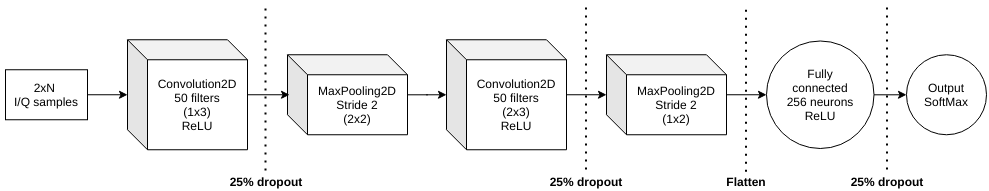
\includegraphics[scale=0.6]{figures/ml_riyaz.png}
  \caption{Representation of the first CNN used}
  \label{fig:cnn-riyaz}
\end{figure}

\textcite{youssef_machine_2017}

\begin{figure}[htbp!]
  \centering
  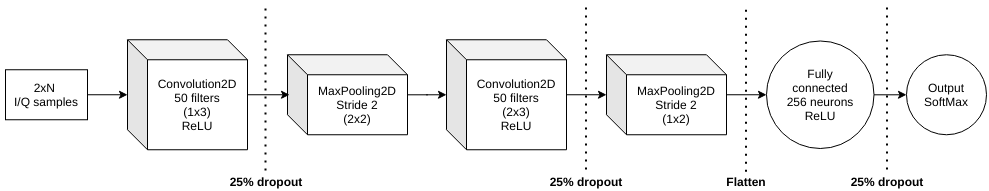
\includegraphics[scale=0.6]{figures/ml_riyaz.png}
  \caption{Representation of the second CNN used}
  \label{fig:cnn-youssef}
\end{figure}

% -------------------------------------------------------------------------------------------------------------
\subsection{Experiments with the first dataset}

Small dataset, simple, airspy HF+

\subsubsection{SVM}

... (If the results are as good as they are with our CNN, we can worry that something is too easy.)

\subsubsection{CNN}

Might not have enough information in signal...

% -------------------------------------------------------------------------------------------------------------
\subsection{Experiments with the more complete dataset}


